\chapter{Resonance Compensation Studies at the CERN Proton Synchrotron Booster}
\label{sec:ch5}

\section{General Description}
The Proton Synchrotron Booster (PSB) is the first circular accelerator in the CERN accelerator complex that ultimately leads to the LHC. Figure \ref{fig:cernac} shows the entire chain of accelerators at CERN, feeding a variety of physics experiments \cite{cernplot}. Following the successful implementation of the LHC Injectors Upgrade (LIU) \cite{liu}, the PSB receives $H^-$ ion beam from the Linac4 at an energy of 160 MeV. Interestingly, the PSB is not just one ring but four identical synchrotron rings stacked on each other. This design counteracts the space charge effects, which are the largest in low-energy machines. Once the ion beam enters the PSB rings, the electrons are stripped off through a charge-exchange process with a carbon foil, and a proton beam is achieved \cite{psbstrip}. The proton beam is then accelerated from an energy of 160 MeV to 2 GeV. Each ring extracts one bunch and is injected in different buckets into the Proton Synchrotron (PS). This description is true for LHC-type beams. Nevertheless, the PSB can also feed protons to other customers such as its highest-intensity user---ISOLDE (Isotope mass Separator On-Line facility) \cite{foteini1}.   

One ring of the PS Booster has a total circumference of 157.08 meters. Multiplying this quantity by the four rings, one gets a length of 628.32 meters, the exact circumference of the next accelerator, the Proton Synchrotron (PS). The PSB has a superperiodicity of 16, meaning it has 16 identical fundamental cells. Each cell has a length of 9.82 meters, housing a sequence of bending magnet, focusing quadrupole, defocusing quadrupole, focusing quadrupole, and bending magnet \cite{tirsithesis,foteinithesis}. Between these main components are drift spaces used for RF insertions, diagnostic devices, injection and extraction devices, and additional multipole corrector magnets. At injection energy, 160 MeV, protons have a revolution period of 1.01 $\mu s$, while at the extraction energy of 2.0 GeV, they have a revolution period of 0.553 $\mu s$. The beam stays in the PS Booster for around 530 microseconds, where CERN and its accelerators are synchronized with a 1.2-second basic period. 

\begin{figure}[H]
    \centering
    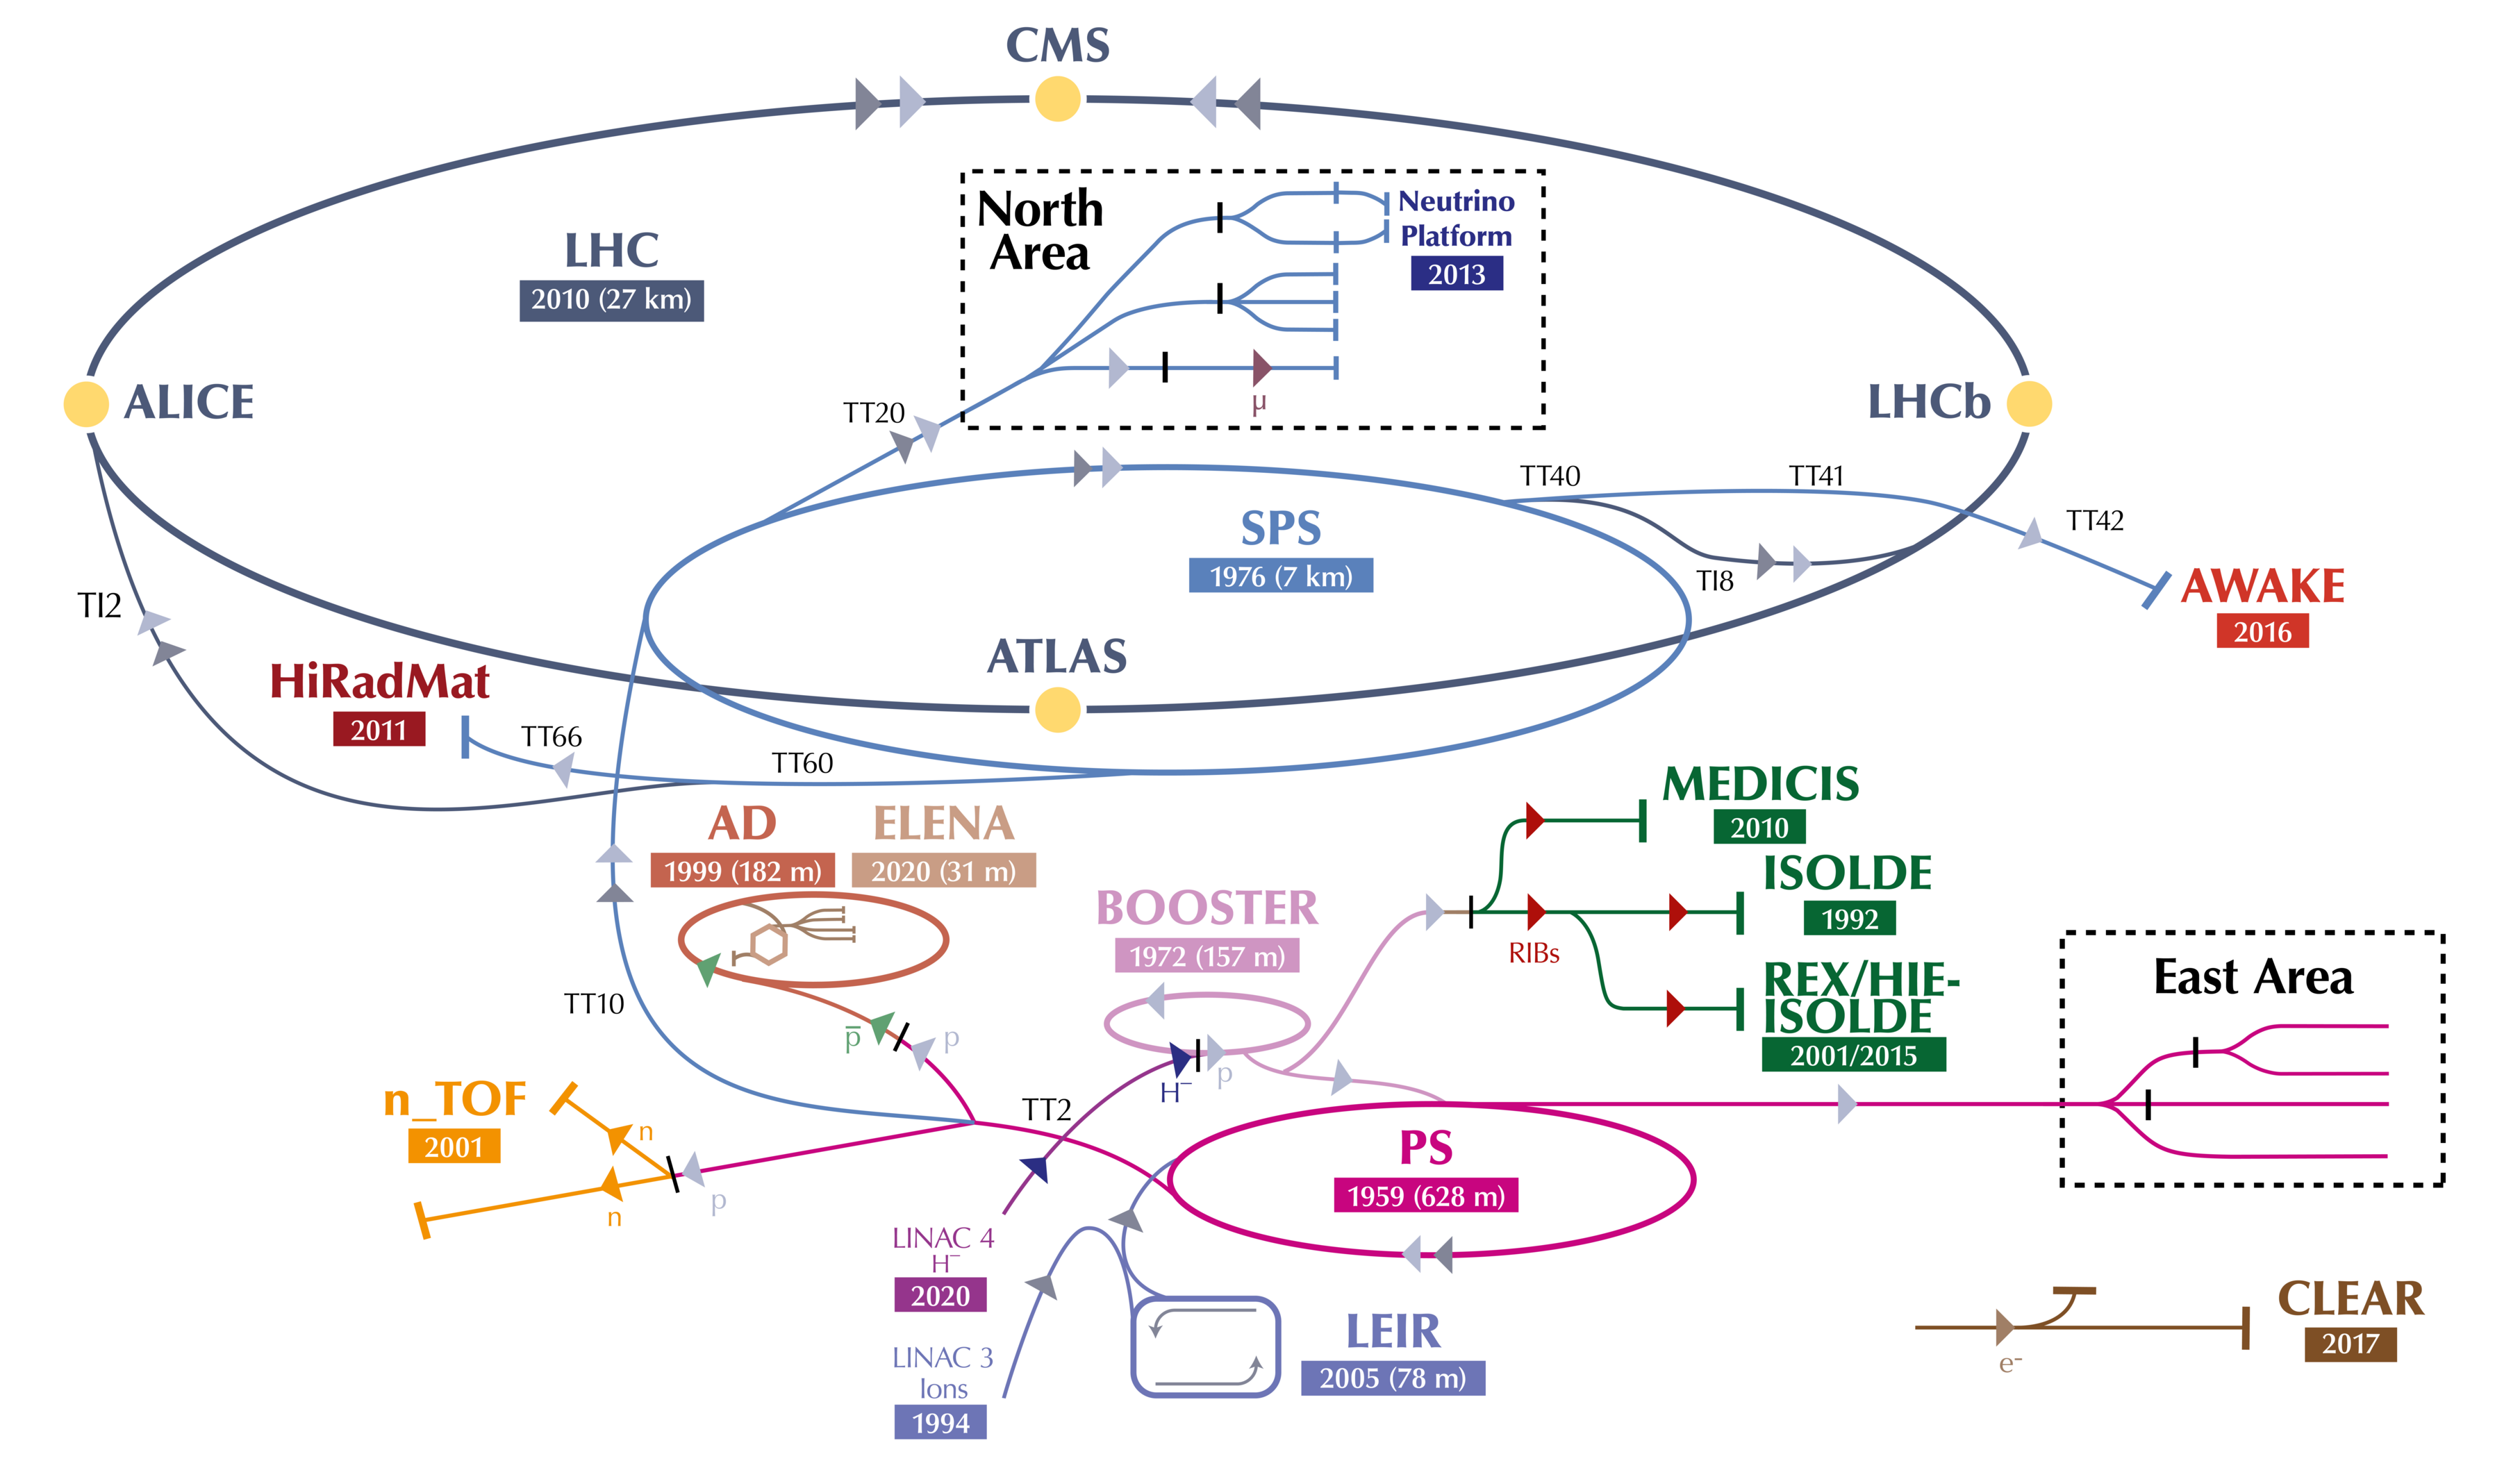
\includegraphics[width=\linewidth]{chapter5/CERN_AC.png}
    \caption{A graphic overview of all accelerators in operation at CERN as of 2022. Original image taken from Ref. \cite{cernplot}. This file is licensed under the Creative Commons Attribution 4.0 International license.}
    \label{fig:cernac}
\end{figure}

\section{Tune Diagram and Operation}

Figure \ref{fig:operational_psb} illustrates the tune diagram dynamics that the LHC-type beam undergoes at the PS Booster \cite{foteini1,foteini2,albright}. As mentioned before, the beam gets injected at an energy of 160 MeV. At this low energy, the tune footprint is large enough that the spread can reach up to 0.5, i.e., $\Delta Q_u \approx -0.5$. The nominal injection tunes are around $Q_x = 4.40$ and $Q_y = 4.45$, in order to accommodate the footprint between the integer resonance lines $Q_u= 4.0$ and the half-integer line $2Q_y=9$. As the beam is accelerated, the quadrupoles are ramped up to match the increasing beam rigidity, but, additionally, a tune ramp is introduced to move the shrinking footprint to a less resonance-populated area in the tune diagram. The nominal extraction tunes are around $Q_x = 4.17$ and $Q_y = 4.23$. At extraction, the beam tune footprint has shrunk by a factor of $(\gamma_L ^3 \beta_L ^2)$, as explained by the beam perveance definition in Eq. \ref{eq:perv}. At extraction, the footprint is smaller than 0.05, i.e., $| \Delta Q_u | \lesssim 0.05$.      

\begin{figure}[H]
    \centering
    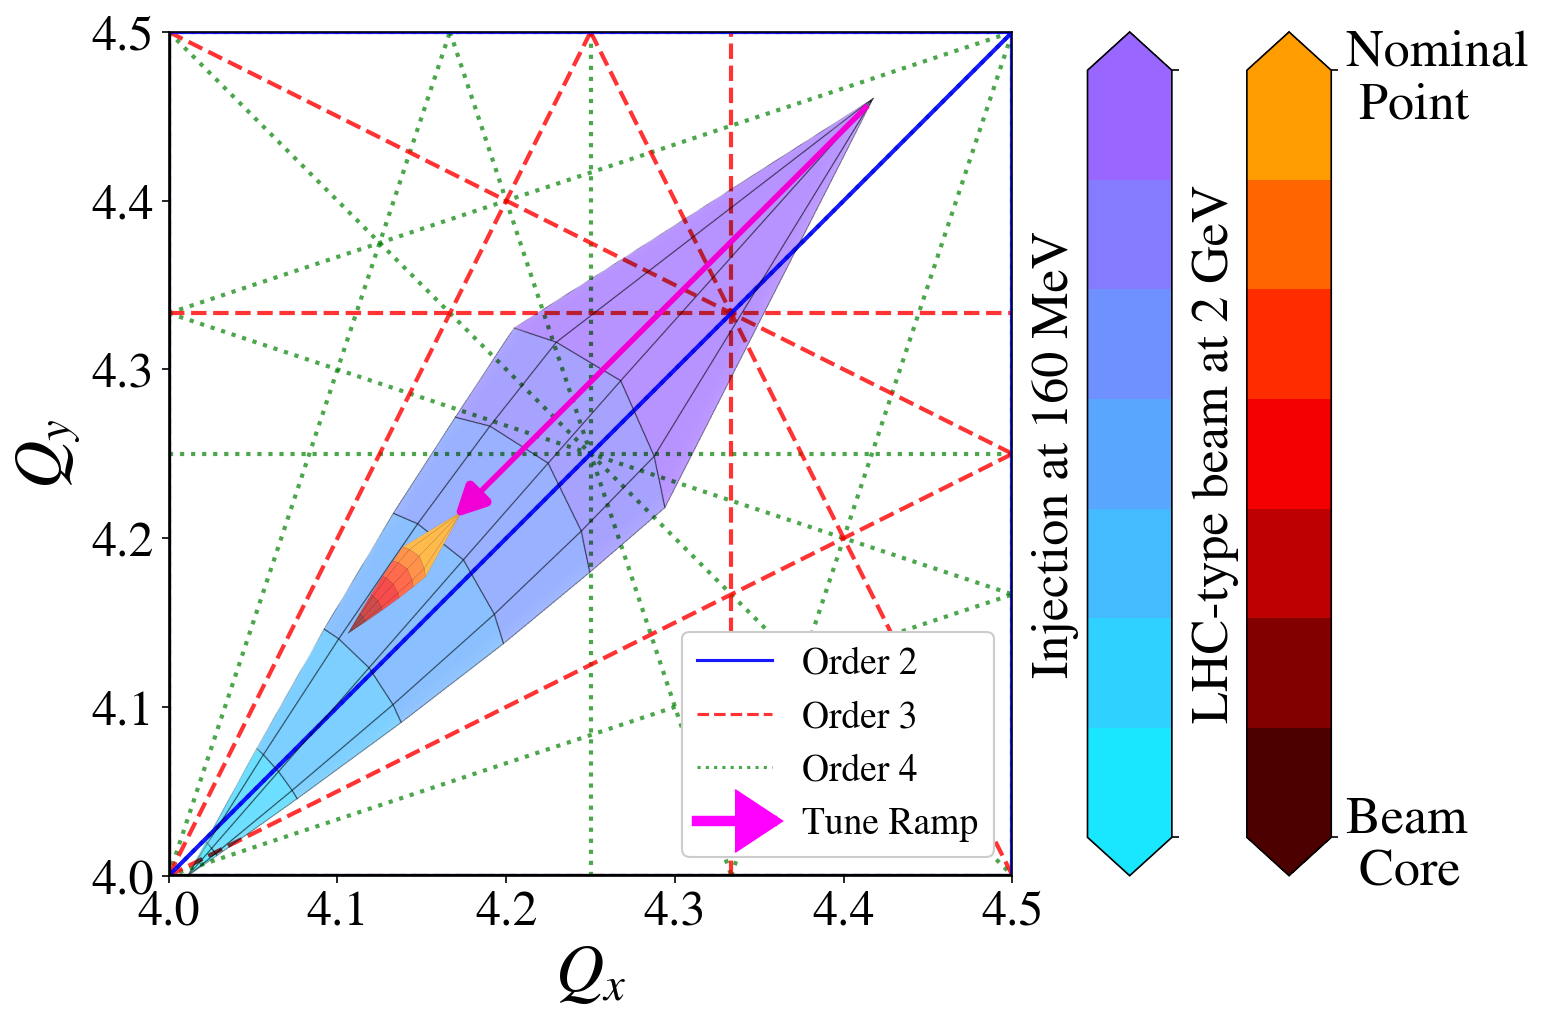
\includegraphics[width=\linewidth,keepaspectratio]{chapter5/operational.png}
    \caption{Operational tune footprint for PSB beam at injection (cool color map) and footprint after the beam has been accelerated to 2 GeV (warm color map). During acceleration, there is a tune ramp illustrated with the fuchsia arrow.}
    \label{fig:operational_psb}
\end{figure}

As illustrated in Fig. \ref{fig:operational_psb} with the fuchsia arrow, the nominal tune ramp crosses several resonance lines. Uncorrected, these resonance lines will lead to beam loss during the tune ramping. These include four third-order resonance lines and four fourth-order lines. It is worth reminding the reader that the third-order lines are excited by sextupole-like components in the ring, while fourth-order lines are excited by octupole-like fields. The third order resonances include two normal sextupole lines, $3Q_x = 13$ and $Q_x+2Q_y = 13$, and two skew sextupole lines, $3Q_y = 13$ and $2Q_x+Q_y = 13$. For the octupole case, these include two normal octupole lines, $4Q_x = 17$ and $Q_x+3Q_y = 17$, two skew octupole lines, $4Q_y = 17$ and $3Q_x+Q_y = 17$, and the octupole coupling sum resonance, $2Q_x +2Q_y =17$. Figure \ref{fig:psbtd} shows all these resonance lines summarized in one tune diagram. All of these resonance lines have different strengths in each Booster ring. It is worth pointing out that the coupling resonance $Q_x - Q_y = 0$ is not strongly excited in the low-intensity operation of the PSB. At higher intensities, it has been demonstrated that this resonance line is driven in fourth-order by space charge \cite{foteinithesis}.

\begin{figure}[H]
    \centering
    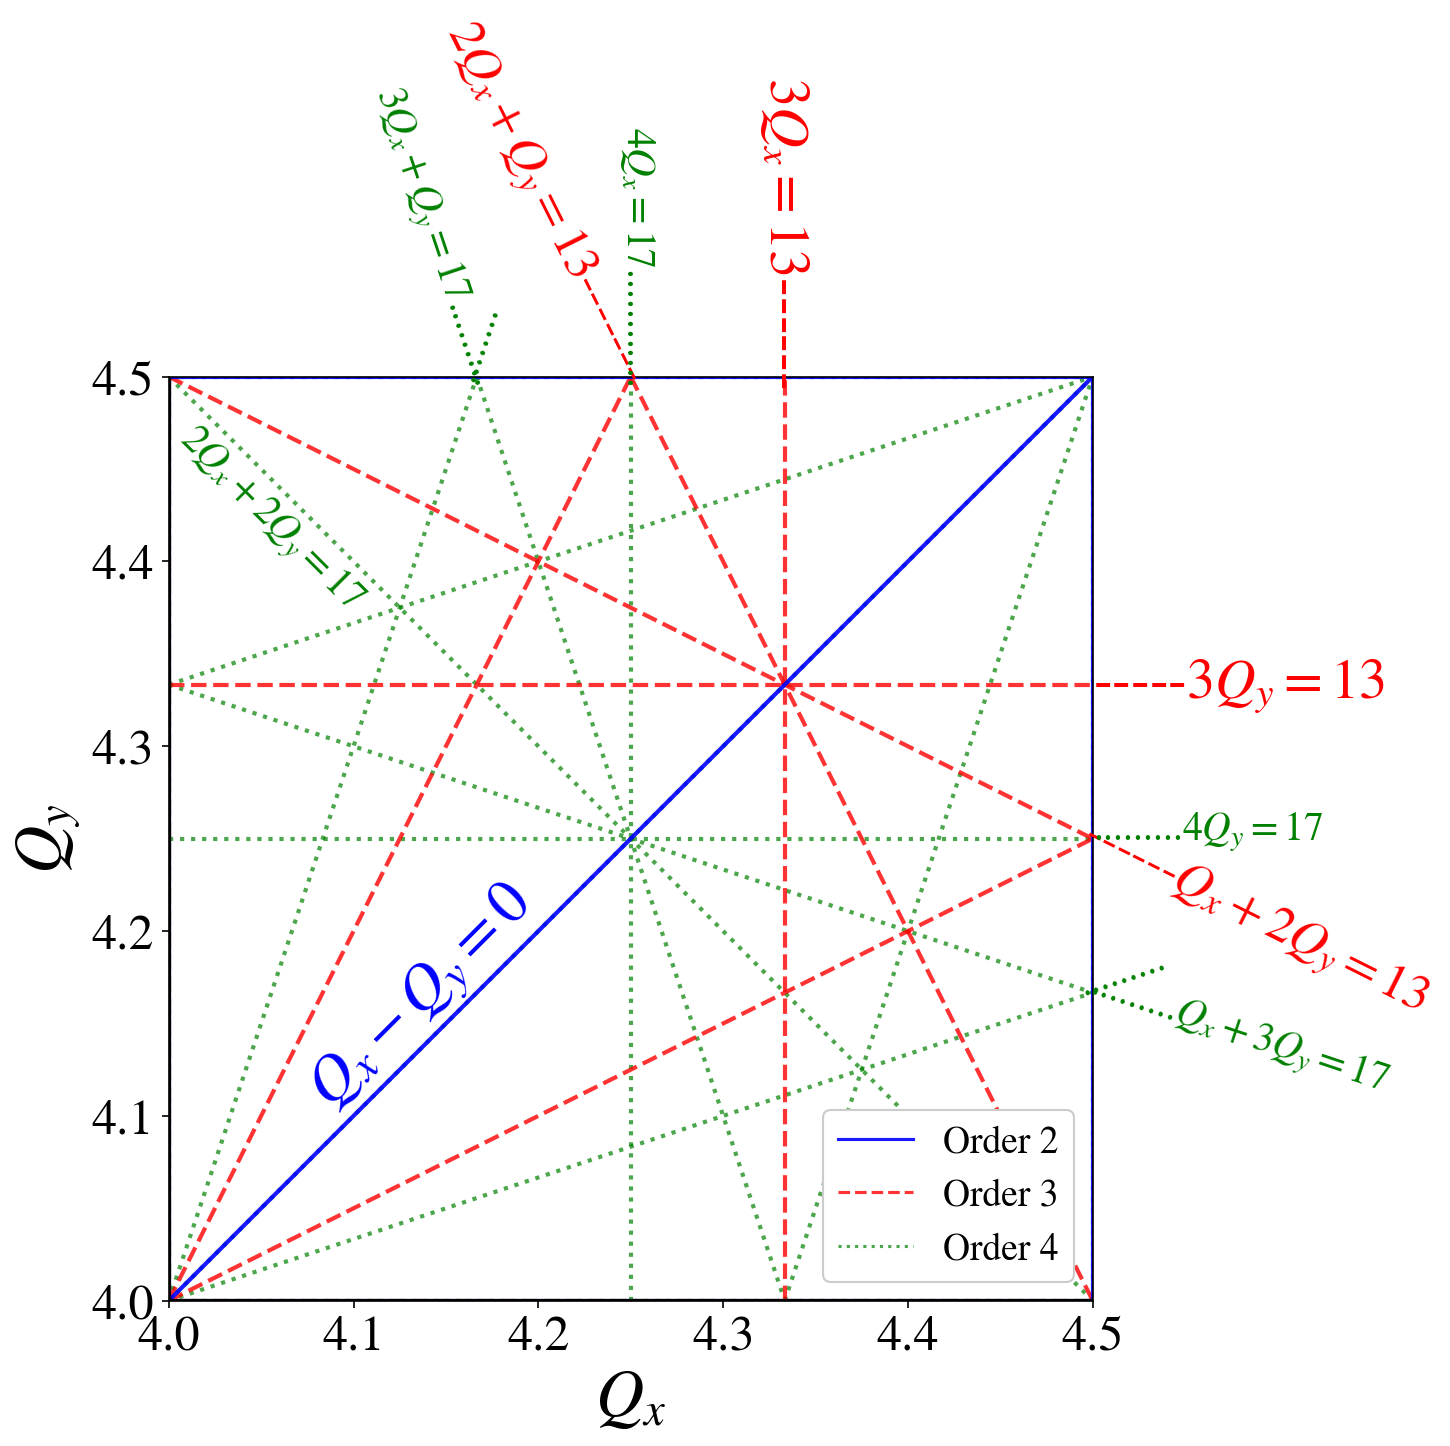
\includegraphics[width=\linewidth]{chapter5/psb_td.png}
    \caption{Portion of the tune diagram enclosing the operational tunes of the PS Booster with relevant resonance lines labeled.}
    \label{fig:psbtd}
\end{figure}

Like the plots shown in Fig. \ref{fig:bare_nocomments} and Fig. \ref{fig:bare_comments}, loss maps can be used to visualize the strength of the resonance lines in the CERN PS Booster. Figure \ref{fig:bare_psb} shows loss maps for each of the four rings in the PSB. These plots are created slightly differently from the ones in the Recycler Ring. The plots shown in Fig. \ref{fig:bare_psb} are an average from four loss maps. One where losses are mapped from (a) left to right, i.e., fixing $Q_y$ and ramping from $Q_x \approx 4.49$ to $Q_x \approx 4.15$, (b) another one from right to left, (c) one from top to bottom, i.e., fixing $Q_x$ and ramping from $Q_y \approx 4.49$ to $Q_y \approx 4.15$, (d) and one from bottom to top. Therefore, these plots show an average from mapping the losses in four directions.    

\begin{figure}[H]
    \centering
    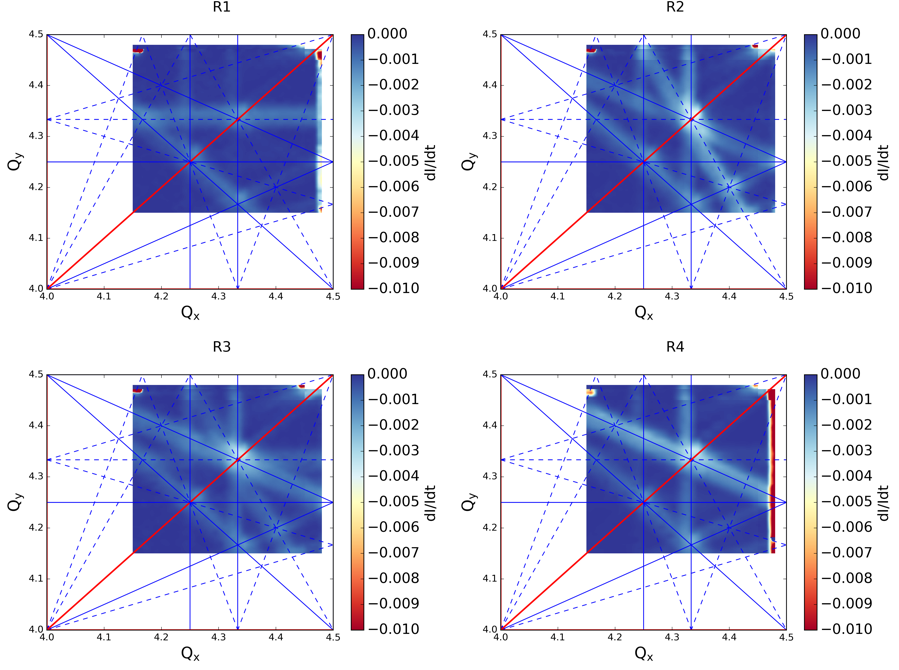
\includegraphics[width=\columnwidth]{chapter5/bare.png}
    \caption{Dynamic loss maps for the bare machine of the four rings (R1, R2, R3, and R4) in the PS Booster. The plots are an average of scanning in 4 directions. Plot provided by F. Asvesta.}
    \label{fig:bare_psb}
\end{figure}

Figure \ref{fig:bare_psb} shows how resonances are excited differently for each ring at the Proton-Synchrotron Booster. For example, third-order lines are more excited for Ring 2 than Ring 1. This feature hints that every ring will have different values for the corrector magnets used for resonance compensation. The fourth-order order skew resonances are not observed in this loss map. The work in the following sections looks to calculate the currents of the corrector magnets used for resonance compensation. This approach involves using two optimization procedures to find the values that clear out the losses from the plots in Fig. \ref{fig:bare_psb}.

\section{Optimization Algorithms for Resonance Compensation}

The whole objective of the following work is to minimize the losses during the PS Booster's operational cycle, as explained in Fig. \ref{fig:operational_psb}. The losses during the cycle come from particles falling on top of third-order and fourth-order resonance lines, as identified in Fig. \ref{fig:psbtd}. In order to decrease the strength of these resonances, sextupoles and octupoles can be used to control their Resonance Driving Terms (RDTs). Nevertheless, measuring and minimizing the RDTs may not always be ideal. For this work, the main observable to optimize was the beam loss from crossing the resonance lines, which is related to the amplitude of the RDTs. Figure \ref{fig:experimentPSB} shows an illustration of the experimental setup used in order to measure this beam loss.

\begin{figure}[H]
    \centering
    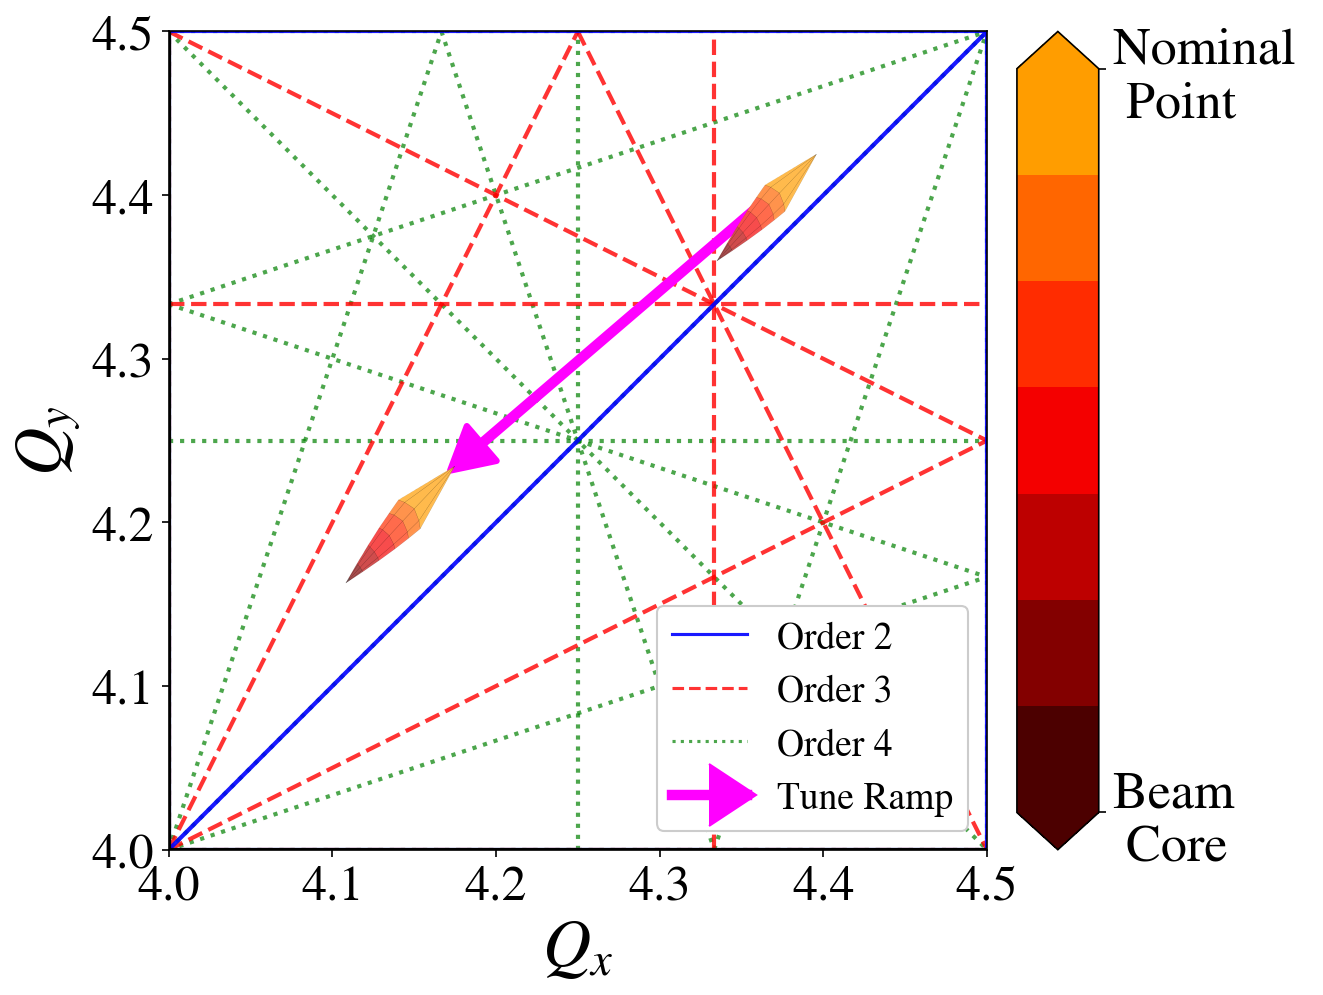
\includegraphics[width=\linewidth]{chapter5/experiment.png}
    \caption{Experimental setup of the tune diagram dynamics for optimizing resonance compensation used in the PS Booster.}
    \label{fig:experimentPSB}
\end{figure}

The experimental setup introduced in the PS Booster involved several steps to find the optimal compensation currents. First, a low-brightness beam was injected into every ring at an energy of 160 MeV. Energy is not ramped up for this configuration, and the machine stays at a flat bottom. Second, a tune ramp was programmed into the quadrupoles in the ring in order to go from initial tunes of $Q_x = 4.40$ and $Q_y = 4.45$ to a final setting of $Q_x = 4.17$ and $Q_y = 4.23$. This particular setting was introduced to mimic the operational tune ramp of the LHC-type beam. The start of this tune ramp occurs within $t_0 = 300$ ms of the start of the cycle and ends at $t_f = 600$ ms, i.e., all of this occurs within a 300 ms time window. During this time window, the beam loss is measured by comparing the beam current at the end of the window to the initial value of the beam current. The currents fed to the corrector magnets remain constant during this measurement. Figures \ref{fig:experimentPSB} and \ref{fig:actorcurrents} summarize this experimental setup. 

While monitoring the beam loss, the corrector magnets used for compensation are varied every cycle according to the optimization algorithm. Table \ref{tab:psbcomp} summarizes the 11 elements used for resonance compensation for this work. Out of these elements, there are 6 normal sextupoles, 3 skew sextupoles, and 2 normal octupoles. Figure \ref{fig:actorcurrents} shows an example of the power cycle in these magnets for one optimization step. Before the tune ramp, most actors show currents at or near zero. As preparation for the tune ramp, the magnets are powered to the set values---per the optimizer calculation. During the tune ramp, they are set to a constant value and powered off once the cycle is finished. These magnets were varied for each ring, and each ring had its independent optimization run. Theoretically, in order to fully correct eight resonance lines, one needs at least 16 correctors. Nevertheless, this work aimed to find a solution to this over-constrained problem through advanced optimization algorithms. 

The two optimization algorithms used were Bayesian Optimization and BOBYQA (Bound Optimization BY Quadratic Approximation). In order to implement these algorithms, the special application GeOFF (Generic Optimization Frontend and Framework) was used \cite{geoff}. This graphical application is designed to facilitate numerical optimization through various algorithms and reinforcement learning on CERN accelerators. It incorporates programmable interfaces that can be used to specify the hyperparameters of the optimization algorithms.  

\begin{table}[H]
    \centering
    \caption{List of elements (optimization actors) in the PS Booster at CERN used for resonance compensation optimization as present in all four PS Booster rings.}
    \label{tab:psbcomp}
    \begin{tabular}{|c|c|c|}
    \hline
    \textbf{Actor} & \textbf{Name} & \textbf{Type}    \\ \hline
    1 & XN04L1    & Normal Sextupole \\ \hline
    2 & XN06L1    & Normal Sextupole \\ \hline
    3 & XN09L1    & Normal Sextupole \\ \hline
    4 & XN012L1    & Normal Sextupole \\ \hline
    5 & XN0311L1    & Normal Sextupole   \\ \hline
    6 & XN0816L1    & Normal Sextupole   \\ \hline
    7 & ON0311L1    & Normal Octupole  \\ \hline
    8 & ON0816L1    & Normal Octupole   \\ \hline
    9 & XSK2L4    & Skew Sextupole  \\ \hline
    10 & XSK4L1    & Skew Sextupole   \\ \hline
    11 & XSK6L4    & Skew Sextupole   \\ \hline
    \end{tabular}
\end{table}

\begin{figure}[H]
    \centering
    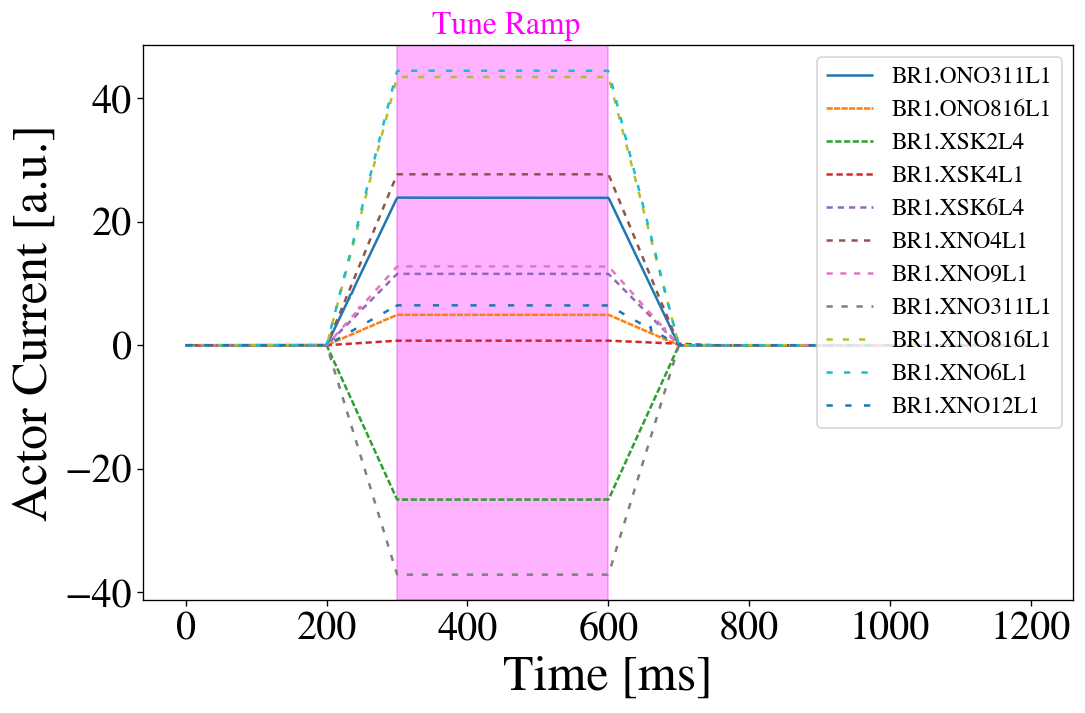
\includegraphics[width=\linewidth]{chapter5/actor_currents.png}
    \caption{Waveform for the currents fed to the correctors (actors) as a function of time in the study cycle for one particular iteration of an arbitrary optimization instance.}
    \label{fig:actorcurrents}
\end{figure}

\subsection{Bayesian Optimization}

Bayesian optimization is a well-established technique used in machine learning and optimization tasks to efficiently search for the optimal solution within a parameter space, particularly when the objective function is expensive or time-consuming to evaluate---this is the case for an accelerator. It combines probabilistic modeling with the principles of Bayesian inference to iteratively update a model of the objective function based on observed data, gradually refining its understanding of the parameter space \cite{bayesian}. By balancing exploration (searching for promising regions) and exploitation (leveraging known information to identify the best areas), Bayesian optimization aims to find the global optimum while minimizing the number of evaluations required. This method is particularly useful in hyperparameter tuning for complex models, where traditional grid search or random search approaches may be impractical due to computational costs.

At the heart of Bayesian optimization are Gaussian processes. A Gaussian process (GP) is a statistical model representing a collection of random variables, any finite subset with a joint Gaussian distribution \cite{bayesian}. GPs are defined by a mean function and a covariance function, which capture prior beliefs about the underlying function being modeled and the correlations between different points in the input space. These special types of statistical models are key to estimating the underlying function that wants to be optimized. Through Bayesian inference, GPs can be updated with observed data, yielding posterior distributions that can inform predictions and lead to an optimized sampling for the Bayesian optimization algorithm. 

Figure \ref{fig:ibo} shows an example of the evolution of the objective function during a Bayesian optimization procedure. In this case, the objective function is the normalized beam loss after the tune ramp illustrated by Fig. \ref{fig:experimentPSB}. It can be seen how the Bayesian optimizer finds solutions that effectively cancel out the beam loss from crossing the resonances. Nevertheless, given that this optimizer is built to find a global minimum, it will keep sampling other regions to ensure the best solution is not a local minimum. The color map of Fig. \ref{fig:ibo} shows how for some of these cases, the optimizer prioritizes exploration and drifts to some unknown region where the losses are high. For these cases, the underlying Gaussian process will learn that there is no worth in exploring these regions. Ultimately, the configuration with the least relative beam loss---the best configuration---is saved and kept as the optimum solution.

\begin{figure}[H]
    \centering
    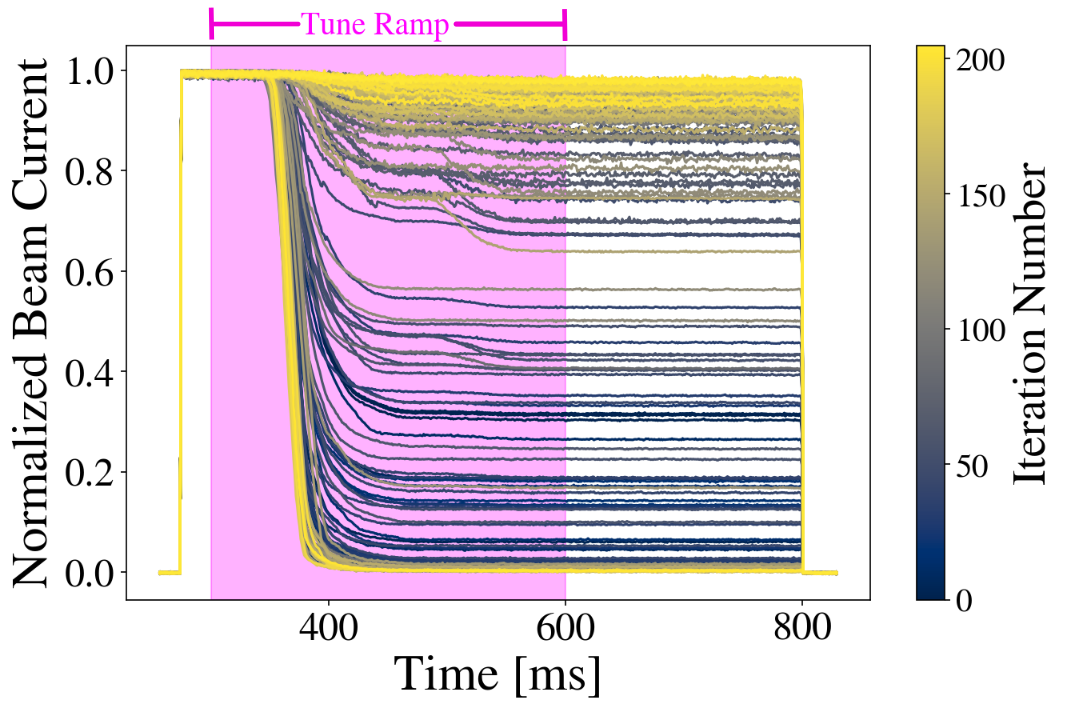
\includegraphics[width=\linewidth]{chapter5/i1_bo_commented.png}
    \caption{Normalized beam current plots for the Bayesian Optimization method done at Ring 1.}
    \label{fig:ibo}
\end{figure}

The bottom plot of Fig. \ref{fig:bo1} shows the explicit steps of each actor versus the number of iterations. Additionally, the top plot shows the trend of the objective function (relative beam loss) as the number of iterations increases. There are significant oscillations in the relative beam loss values, especially at the beginning, but a general trend towards minimization as the algorithm progresses through iterations. The early iterations reflect the exploration phase. BO is sampling points that give a broad understanding of the objective function's landscape. As iterations progress, there is a trend toward certain regions in the parameter space. This trend indicates a shift from exploration to exploitation, where the algorithm samples more from areas it believes to be near the optimum. The narrowing of actor current variability suggests a reduction in uncertainty about the location of the minimum beam loss. The GP model is becoming more informed and better trained. At the end of the optimization instance, such as the one shown in Fig. \ref{fig:bo1}, the configuration that gave the smallest relative beam loss is saved. GeOFF sets the default configuration of the correctors to these best values. 

The corrector values for the best configurations are important to discuss from Fig. \ref{fig:bo1}. It can be seen from Fig. \ref{fig:bo1} that some correctors land on the limit values, e.g., the limits for the normal sextupoles (XNO magnets) were [-50,50]. This behavior is especially apparent for the octupole correctors (ONO magnets), which have limits from -80 to 80, e.g., the magnet ONO816L1 is maxed out. Nevertheless, this was expected given that only two octupole correctors were used to correct four fourth-order lines, whereas one would need eight correctors to cancel out all the fourth-order RDTs fully. It is important to remind the reader that to implement these types of algorithms with several actors efficiently, the currents need to be normalized between [0,1] to ensure that all the data is on the same scale and improve the model performance. This procedure is done by GeOFF internally.    

\begin{figure}[H]
    \centering
    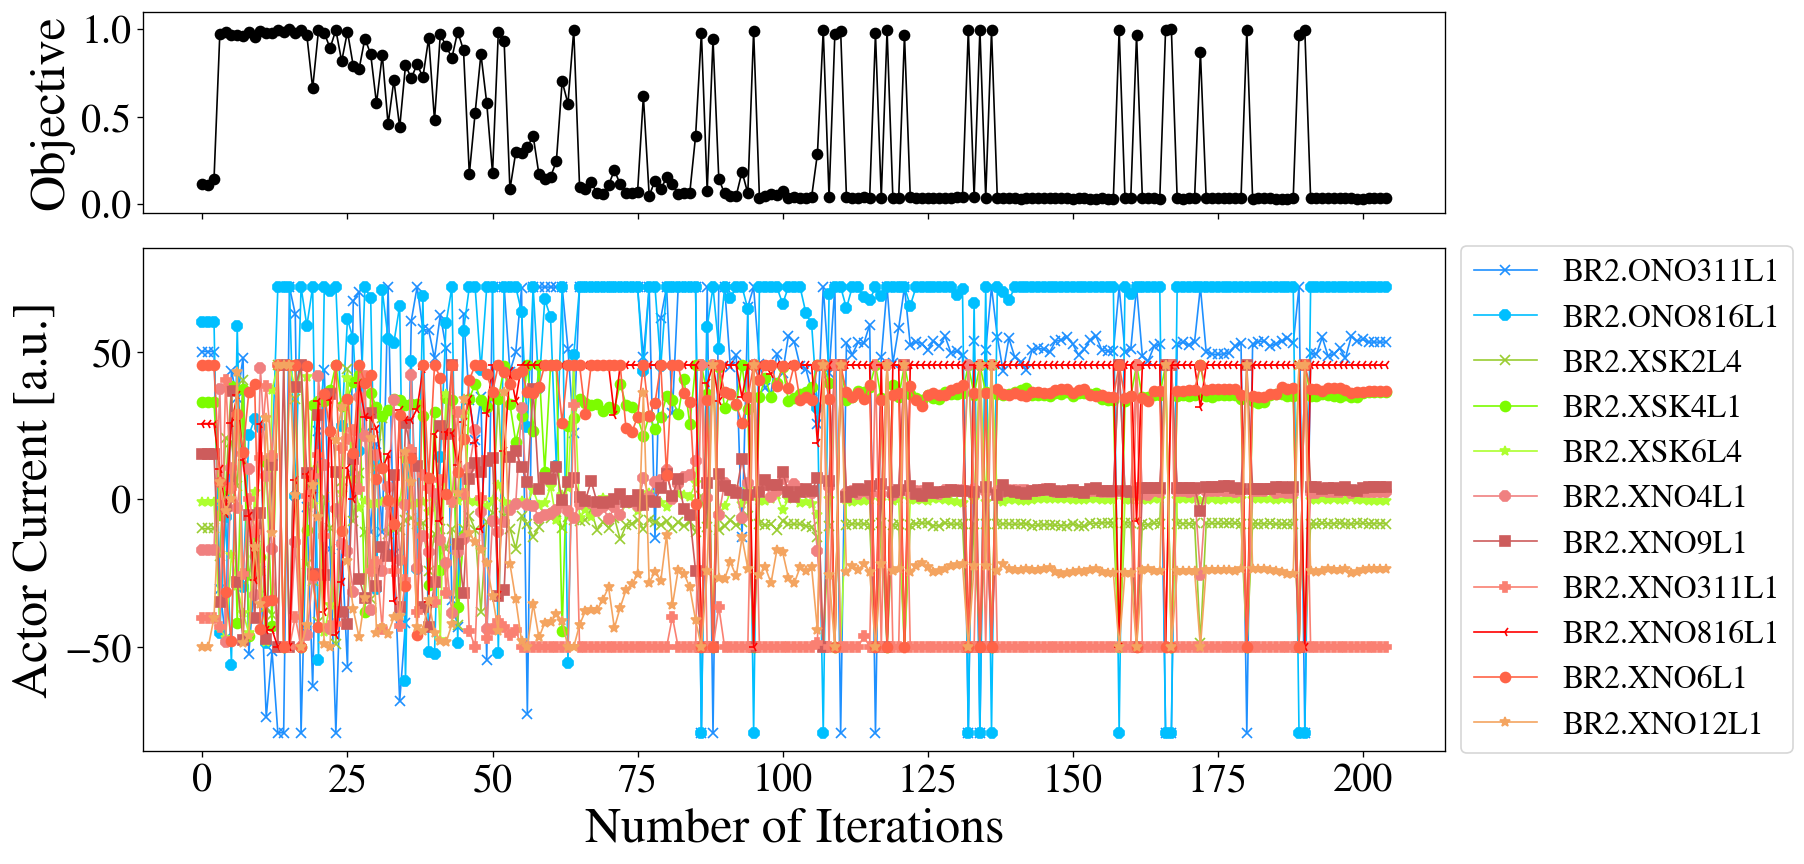
\includegraphics[width=\linewidth]{chapter5/2023_05_02_R2_LHCramp_BayesOpt.png}
    \caption{Summary for Bayesian optimization of resonance compensation applied to Ring 2 in the CERN PSB.}
    \label{fig:bo1}
\end{figure}

While Fig. \ref{fig:bo1} shows a relatively smooth Bayesian optimization instance for Ring 2, Figs. \ref{fig:bo21} and \ref{fig:bo22} show a different story for Ring 3. This particular optimization instance failed to find a configuration yielding a relative beam loss of less than 5\% after 200 iterations---unacceptable for operation. This feature can be seen on the top plot of Fig. \ref{fig:bo21}, which follows the objective function across iterations. In order to find an acceptable configuration, the BO instance was performed again, but in this case, the initial Gaussian process was trained with the data from the previous incomplete run. The additional 350 iterations from this second instance are shown in Fig. \ref{fig:bo22}. This second instance yielded configurations that led to acceptable values for the relative beam loss. Possible explanations for this hurdle include inadequate exploration of the parameter space, poor choice of the kernel for the Gaussian Process, poor choice of hyperparameters for this BO, and noise in the measurements.

\begin{figure}[H]
    \centering
    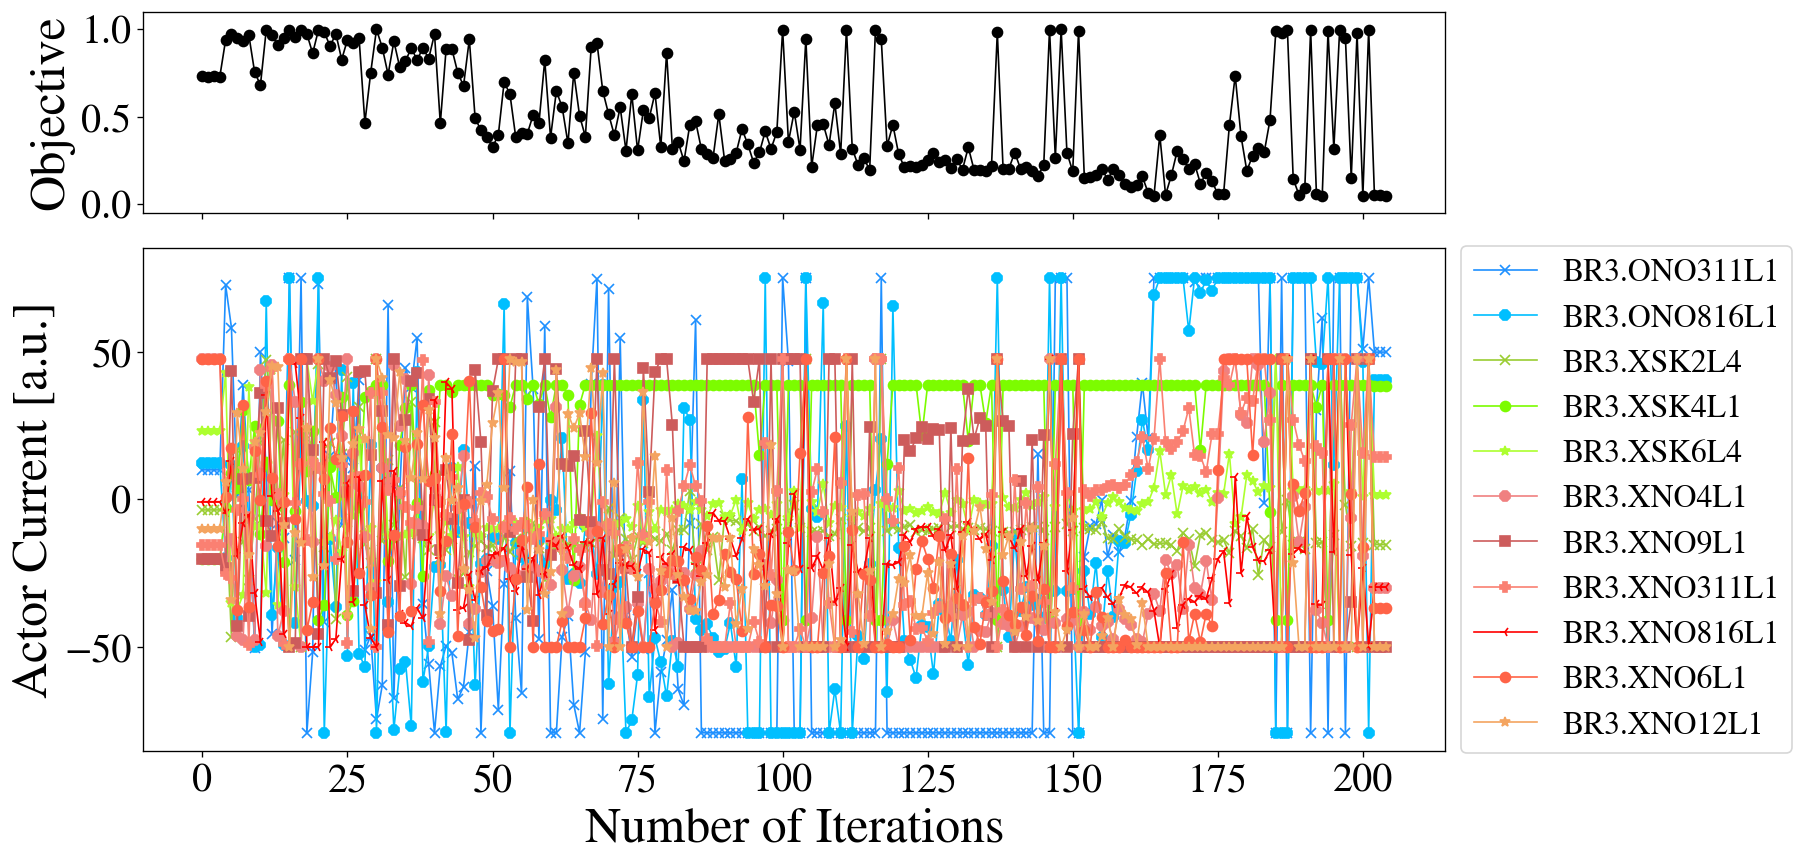
\includegraphics[width=\linewidth]{chapter5/2023_05_02_R3_LHCramp_BayesOpt.png}
    \caption{Summary for the first instance of Bayesian optimization towards resonance compensation applied to Ring 3 in the CERN PSB.}
    \label{fig:bo21}
\end{figure}

\begin{figure}[H]
    \centering
    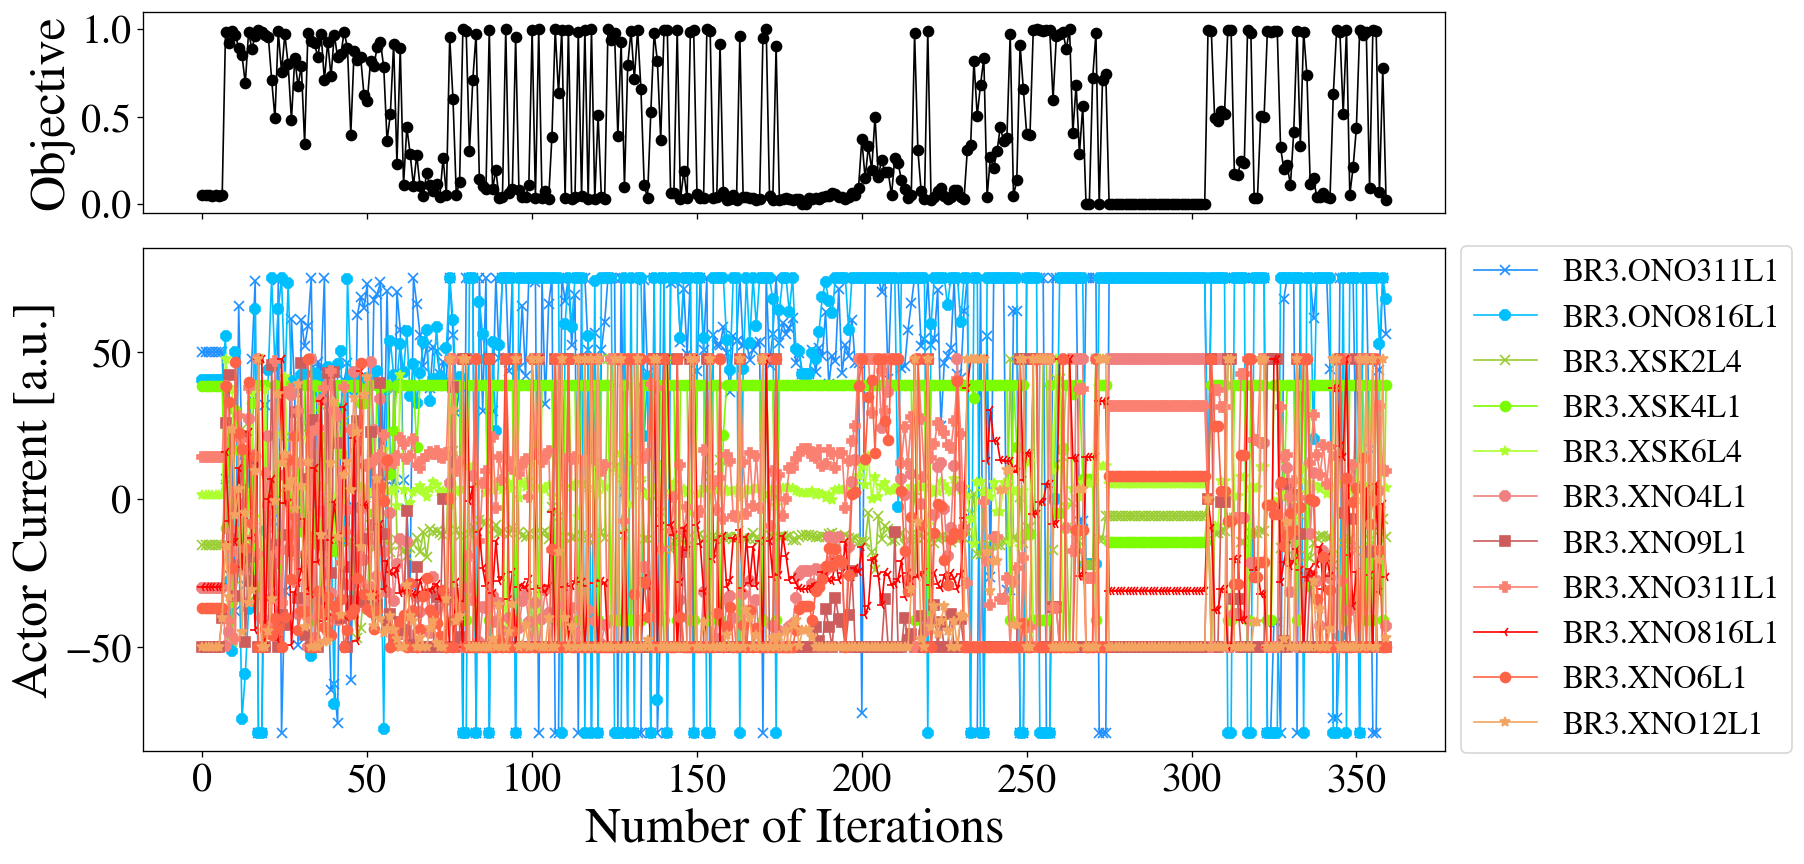
\includegraphics[width=\linewidth]{chapter5/2023_05_02_R3_LHCramp_BayesOpt_itrtn2.png}
    \caption{Summary for the second instance of Bayesian optimization of resonance compensation applied to Ring 3 in the CERN PSB. This second optimization instance was trained with the data from the first instance.}
    \label{fig:bo22}
\end{figure}

\subsection{BOBYQA (Bound Optimization BY Quadratic Approximation)}

BOBYQA, which stands for Bound Optimization BY Quadratic Approximation, is an optimization algorithm commonly used for solving constrained optimization problems \cite{bobyqa}. Unlike gradient-based methods, BOBYQA belongs to the class of derivative-free optimization algorithms, making it suitable for scenarios where the objective function is not differentiable or computationally expensive to evaluate. The algorithm iteratively builds a quadratic approximation of the objective function within a trust region, a bounded area around the current solution. By iteratively updating the quadratic model and moving towards the predicted optimum within the trust region, BOBYQA efficiently explores the search space while minimizing the number of function evaluations. It employs a bound constraint strategy to ensure that the search remains within specified bounds. In this case, BOBYQA was used to solve the same optimization task from the last section but using a special type of beam at the PSB, the BCMS (Bunch Compression Merging and Splitting) beam. 

The BCMS configuration is special given that it is produced with a smaller intensity (compared to the LHC-type beam from the previous section), and, hence, it has a smaller tune spread. For this case, the injection tunes were changed from those shown in Fig. \ref{fig:experimentPSB}. The injection tunes were chosen to avoid one normal sextupole and one skew-sextupole resonance. This different configuration changes the optimum compensation currents compared to the Bayesian optimization results.

Similar to the exercise done in Fig. \ref{fig:ibo}, Fig. \ref{fig:ibobyqa} shows the relative beam loss profiles for an instance of the  BOBYQA optimization done on Ring 1. As the iterations progress (transitioning from blue to yellow), the spread in beam current values decreases. This decrease suggests that the algorithm is refining its search based on the feedback from the objective function and moving towards regions of the parameter space that yield better optimization results. The later iterations, indicated by yellow lines, show beam current trajectories closer together. This convergence pattern signifies that the algorithm has likely identified a promising region in the parameter space and is now fine-tuning the parameters. It minimizes the variance between iterations, suggesting an approach toward a stable solution.

\begin{figure}[H]
    \centering
    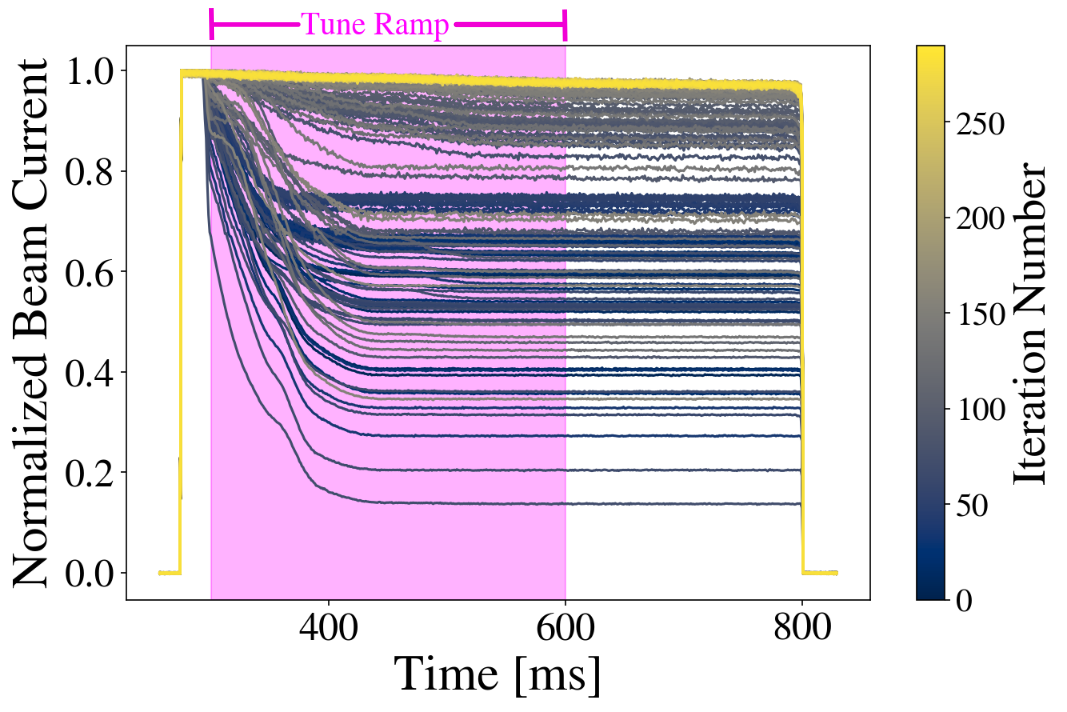
\includegraphics[width=\linewidth]{chapter5/i2_bobyqa_commented.png}
    \caption{Normalized beam current plots for the BOBYQA method done at Ring 1.}
    \label{fig:ibobyqa}
\end{figure}

Similar to the exercise done for the Bayesian optimization, Fig. \ref{fig:bobyqa1} shows the evolution of the objective function and actor currents for a BOBYQA optimization instance on a BCMS beam. The initial values were set from the Bayesian optimization results for each ring, as discussed in the last section. The trend of the objective function (top plot) shows a general decrease in relative beam loss as the number of iterations increases, indicating that the optimization successfully finds parameters that result in less beam loss. The bottom graph illustrates the variation of the actor currents in arbitrary units across iterations. A unique line pattern and color distinguish each actor. Some correctors are kept at 0, given that they were unavailable for Ring 3. Implementing BOBYQA through GeOFF ensures the algorithm does not fall to a local minimum by bumping the settings to a new configuration once it falls to a stable one. That can be seen from the sudden oscillations in the objective function plot from Fig. \ref{fig:bobyqa1}.  

\begin{figure}[H]
    \centering
    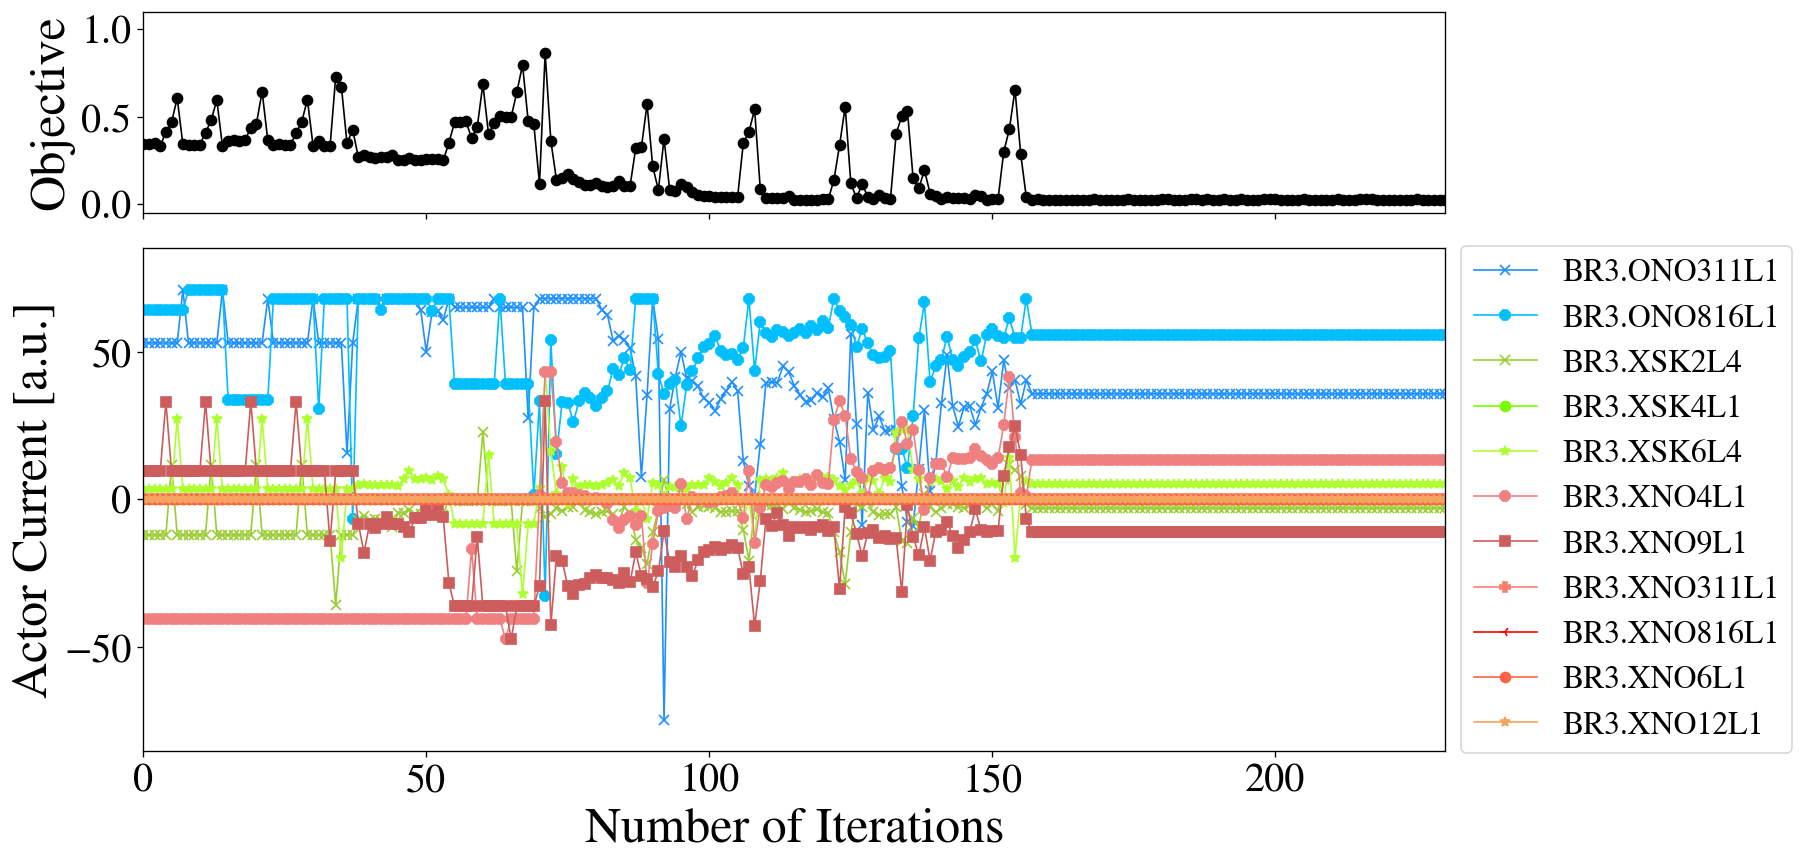
\includegraphics[width=\linewidth]{chapter5/2023_05_04_R3_BCMS_bobyqa.png}
    \caption{Summary for BOBYQA optimization of resonance compensation applied to Ring 3 in the CERN PSB for BCMS (Bunch Compression Merging and Splitting) beam.}
    \label{fig:bobyqa1}
\end{figure}

Comparing this BOBYQA instance with the Bayesian optimization results, one can see that the exploration phase is much shorter and less broad for the BOBYQA instance. Similarly, the variation steps from BOBYQA in the actor currents are smaller than BO. This comparison is true because of the underlying mechanism used to estimate the objective function and its uncertainty. BOBYQA uses deterministic local quadratic models, while Bayesian Optimization uses probabilistic models that measure uncertainty. BOBYQA is generally considered a local search technique, meaning it may be more prone to finding a local minimum than a global minimum. Hence, the initial point for BOBYQA holds more importance. Bayesian optimization is generally used for global optimization and is particularly strong in high-dimensional spaces or when function evaluations are very expensive. In summary, while both algorithms are powerful tools for optimization in accelerator physics problems, the choice between BOBYQA and Bayesian optimization will depend on the specific characteristics of the problem at hand, including the nature of the objective function, the presence of constraints, the dimensionality of the problem, practical considerations like the availability of computational and experimental resources, and, ultimately, availability of study/machine development time.  

\section{Experimental Verification of Compensation}

The whole point of the optimization algorithms explained in the last sections was to reduce the losses that show up in the loss map from Fig. \ref{fig:bare_psb}. Figure \ref{fig:bocomp_psb} shows a new loss map with the best configurations found for each ring using the Bayesian optimization procedure on LHC-type beam. When comparing both loss maps, it is clear that with these new configurations, the loss maps have been cleared out of losses in the region of interest. The immediate losses are decreased by nearly one order of magnitude in the region occupied by the tune ramp. In particular, these new configurations largely suppress the third-order resonances that dominated the losses in Fig \ref{fig:bare_psb}. Nevertheless, some resonance lines are still visible in the loss maps in Fig. \ref{fig:bocomp_psb}, e.g., $Q_x - 2 Q_y = -4$. Given that these lines are not in the region of PSB operation, they are not of particular concern. 

This chapter has shown a different approach to resonance compensation from the one presented in Ch. \ref{sec:ch4}. Chapter \ref{sec:ch4} showed a physics-informed approach by minimizing the Recycler's RDTs and, ultimately, leading to the reduction of beam loss. On the other hand, the previous sections of this chapter showed an optimization-based approach, which can be considered a brute-force line of action. In this approach, all the actors are thrown into an optimization algorithm, which finds a numerical solution that minimizes the objective function. There is no physics involved, just numerical optimization. In particular, BOBYQA's deterministic approach can quickly determine a solution when the accelerator operates near a resonance compensation optimum. With its probabilistic nature, Bayesian Optimization is better suited for exploring unknown or poorly understood operational regimes. All the previous approaches have been proven to work and yield satisfactory results in the context of resonance compensation. The choice between optimization-based and physics-informed approaches—--or a combination thereof—--depends on the specific context of the particle accelerator's operational goals, the available data, and the accuracy of the model.

\begin{figure}[H]
    \centering
    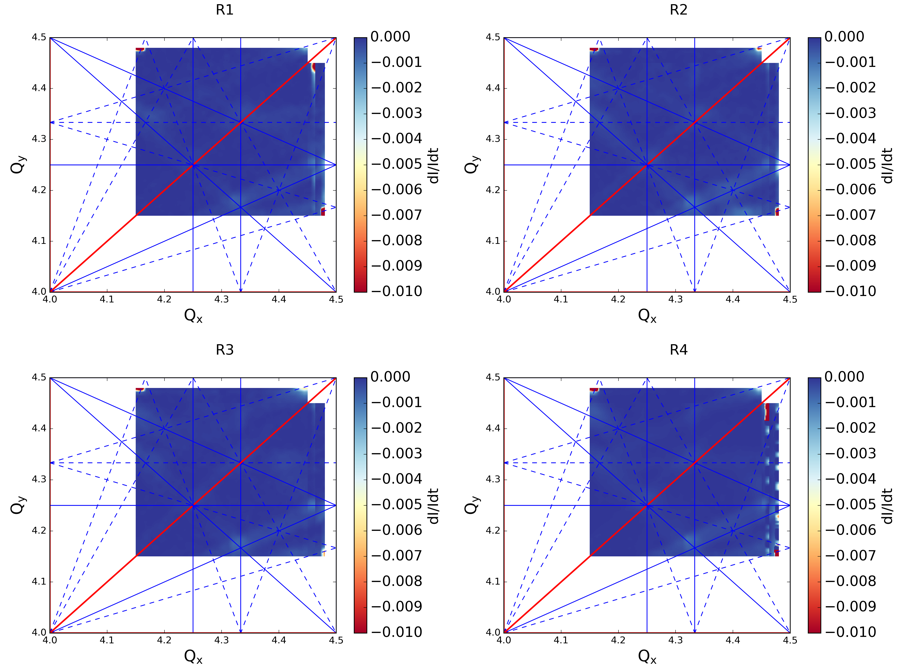
\includegraphics[width=\columnwidth]{chapter5/bocomp.png}
    \caption{Dynamic loss maps for the four rings in the PS Booster with the best configuration from the Bayesian optimization of the resonance compensation. The plots are an average of scanning in 4 directions. Plot provided by F. Asvesta.}
    \label{fig:bocomp_psb}
\end{figure}
